\documentclass[tikz]{standalone}
  \usetikzlibrary{calc}
\begin{document}
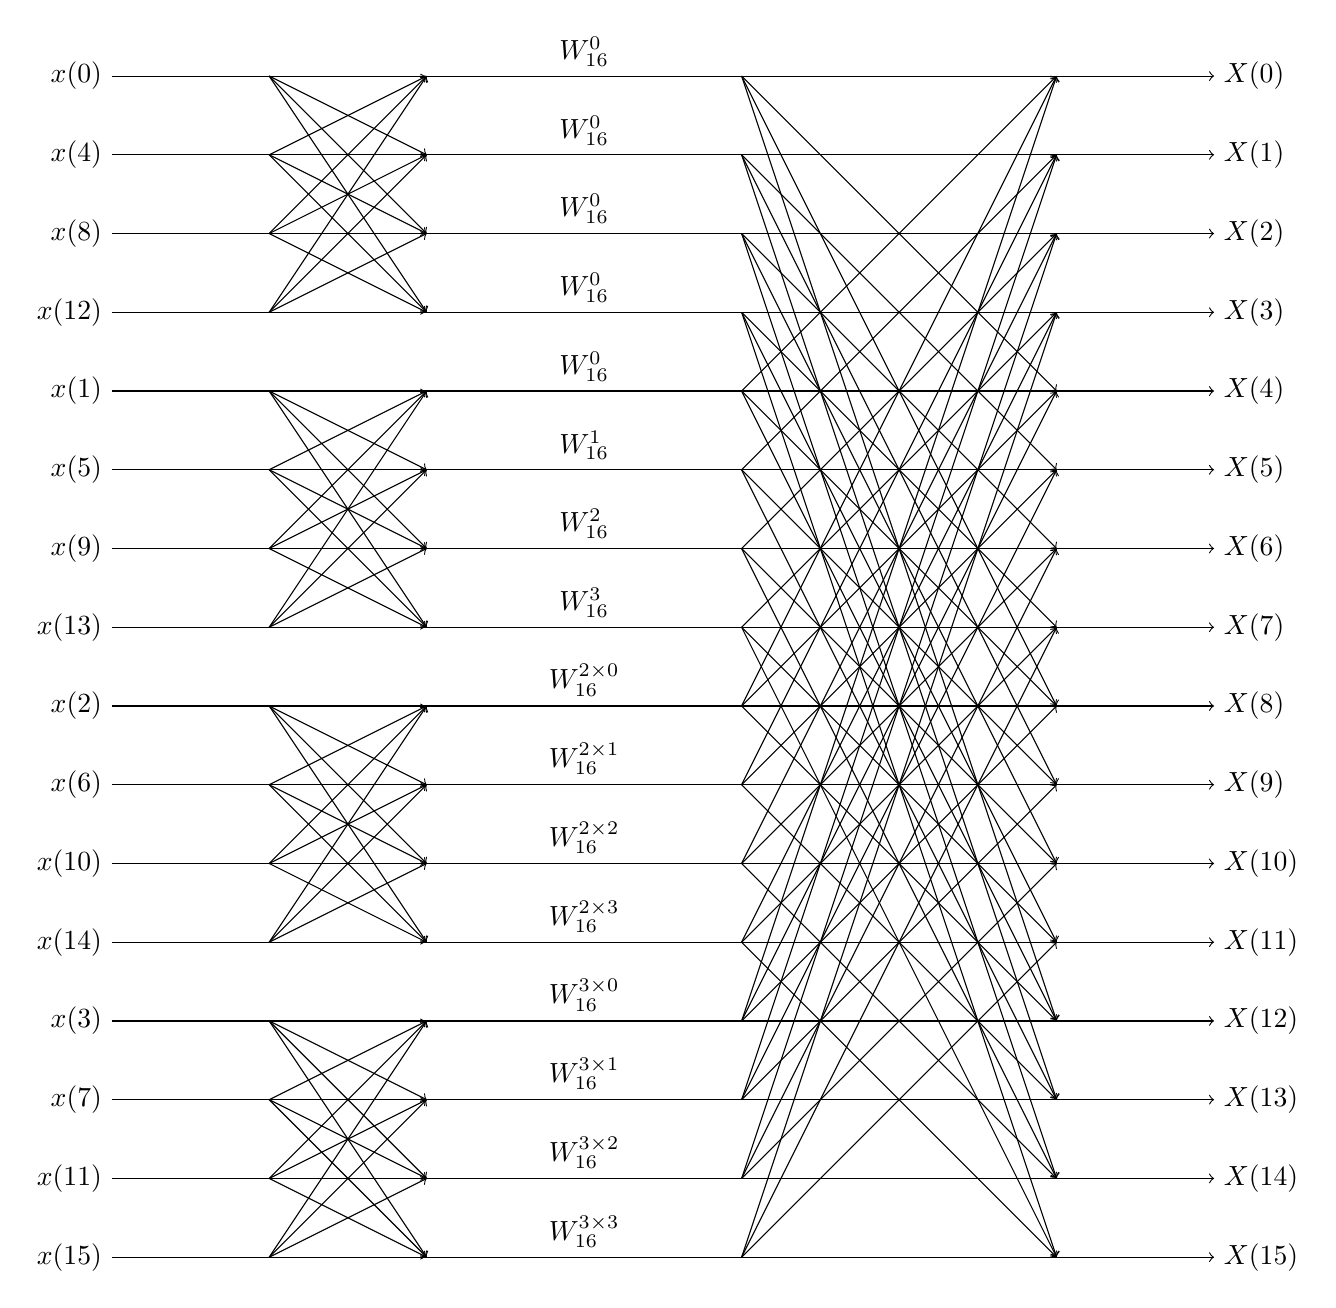
\begin{tikzpicture}
  % input
  \foreach \x/\inx in {0/0, 1/4, 2/8, 3/12, 4/1, 5/5, 6/9, 7/13, 8/2, 9/6, 10/10, 11/14, 12/3, 13/7, 14/11, 15/15}
  \draw[->] (0, 15-\x) node[anchor=east]{$x(\inx)$} -- (2, 15-\x) -- (14 ,15-\x);
  % output
  \foreach \x in {0,...,15}
  \draw (14 ,15-\x) node[anchor=west]{$X(\x)$};
  % layer 1
  \foreach \x in {0, 4, 8, 12}
    {
      \draw[->] (2, 15-\x)    -- (4, 15-\x-3);
      \draw[->] (2, 15-\x)    -- (4, 15-\x-2);
      \draw[->] (2, 15-\x)    -- (4, 15-\x-1);
      \draw[->] (2, 15-\x-1)  -- (4, 15-\x-2);
      \draw[->] (2, 15-\x-1)  -- (4, 15-\x);
      \draw[->] (2, 15-\x-1)  -- (4, 15-\x-3);
      \draw[->] (2, 15-\x-2)  -- (4, 15-\x-1);
      \draw[->] (2, 15-\x-2)  -- (4, 15-\x-3);
      \draw[->] (2, 15-\x-2)  -- (4, 15-\x);
      \draw[->] (2, 15-\x-3)  -- (4, 15-\x);
      \draw[->] (2, 15-\x-3)  -- (4, 15-\x-2);
      \draw[->] (2, 15-\x-3)  -- (4, 15-\x-1);
    }
  \draw (6, 15-0) node[anchor=south]{$W_{16}^{0}$};
  \draw (6, 15-1) node[anchor=south]{$W_{16}^{0}$};
  \draw (6, 15-2) node[anchor=south]{$W_{16}^{0}$};
  \draw (6, 15-3) node[anchor=south]{$W_{16}^{0}$};
  \draw (6, 15-4) node[anchor=south]{$W_{16}^{0}$};
  \draw (6, 15-5) node[anchor=south]{$W_{16}^{1}$};
  \draw (6, 15-6) node[anchor=south]{$W_{16}^{2}$};
  \draw (6, 15-7) node[anchor=south]{$W_{16}^{3}$};
  \draw (6, 15-8) node[anchor=south]{$W_{16}^{2 \times 0}$};
  \draw (6, 15-9) node[anchor=south]{$W_{16}^{2 \times 1}$};
  \draw (6, 15-10) node[anchor=south]{$W_{16}^{2 \times 2}$};
  \draw (6, 15-11) node[anchor=south]{$W_{16}^{2 \times 3}$};
  \draw (6, 15-12) node[anchor=south]{$W_{16}^{3 \times 0}$};
  \draw (6, 15-13) node[anchor=south]{$W_{16}^{3 \times 1}$};
  \draw (6, 15-14) node[anchor=south]{$W_{16}^{3 \times 2}$};
  \draw (6, 15-15) node[anchor=south]{$W_{16}^{3 \times 3}$};
  % layer 2
  \foreach \x in {0, 1, 2, 3}
    {
      \draw[->] (8, 15-\x)     -- (12, 15-\x-4);
      \draw[->] (8, 15-\x)     -- (12, 15-\x-8);
      \draw[->] (8, 15-\x)     -- (12, 15-\x-12);
      \draw[->] (8, 15-\x-4)   -- (12, 15-\x);
      \draw[->] (8, 15-\x-4)   -- (12, 15-\x-8);
      \draw[->] (8, 15-\x-4)   -- (12, 15-\x-12);
      \draw[->] (8, 15-\x-8)   -- (12, 15-\x);
      \draw[->] (8, 15-\x-8)   -- (12, 15-\x-4);
      \draw[->] (8, 15-\x-8)   -- (12, 15-\x-12);
      \draw[->] (8, 15-\x-12)  -- (12, 15-\x);
      \draw[->] (8, 15-\x-12)  -- (12, 15-\x-4);
      \draw[->] (8, 15-\x-12)  -- (12, 15-\x-8);
    }

\end{tikzpicture}
\end{document}